\documentclass[12pt]{article}

\usepackage[utf8]{inputenc}
\usepackage{fancyhdr}
\usepackage{xcolor,graphicx}
\usepackage{fancyvrb}
\usepackage{tcolorbox}

% Allow explicit linebreaks in table items
\usepackage{makecell}

% Allow tables to span page boundaries.
\usepackage{longtable}
\setlength{\LTpre}{5pt}
\setlength{\LTpost}{5pt}

\pagestyle{fancy}

%\lhead{Parallel Computing with LMGC90}
\chead{}
\rhead{} 
\lfoot{}
\cfoot{}
\rfoot{\hfill \thepage}
\renewcommand{\headrulewidth}{0pt}

\fancypagestyle{mypagestyle}{%
\lhead{}
\chead{}
\rhead{} 
\lfoot{}
\cfoot{}
\rfoot{\hfill \thepage}
}

% No indent text 
\setlength\parindent{0pt}
\setlength\parskip{1mm plus 1mm}

% Space between paragraphs
\setlength{\parskip}{2.0\parskip}

%%%%%%%%%%%%%%%%%%%%%%%%%%%%%%%%%%%%%%%%%%%%%
%%%%%%%%%%%%%%%%%%%%%%%%%%%%%%%%%%%%%%%%%%%%%
%%%%%%%%%%%%%%%%%%%%%%%%%%%%%%%%%%%%%%%%%%%%%

\begin{document}

\thispagestyle{mypagestyle}

\begin{center}
  \textbf{\Large Parallel computing with LMGC90 hahahahahah}\\
  \today
\end{center}

\section*{Introduction}
Part of the developments of LMGC90 are currently dealing with the optimization of tasks using parallel computing. However, given the complexity of the code and the structure of the Contact Dynamics Method (i.e., the algorithm behinds LMGC90), not all the can be coded for multithreading processing.

Between the most time-consuming operations the code runs, we find on top: 1) the solver of interactions (the resolution of contact forces and particles’ velocities), and 2) the contact detection. The first is parallelized but not the second.

Other parts of the code, such as the reading/writing of files, the preparation of the simulation (this is the computation of rigid body properties, external forces) are not parallelized either. 

Now, how many processors is it worth using with LMGC90? Bellow, you find a figure from the Ph.D. dissertation of Mathieu Renouf (Optimisation numérique et calcul parallèle pour l’étude de milieux divisés bi- et tridimensionnels, 2004) presenting the speed-up (SP) of LMGC90 as a function of the number of processors (P). 
The different lines correspond to different data structures the code can use. For the moment, the most stable and that we usually use is the SDL (“Stored Delassus Loops”). 
As you can see, the speed-up quickly reaches a plateau around 4. 
That means that, at most, we can divide the computing time by 4 times when using around 16 processors. It is probably not worth using 16 processors for just a speed-up of 4 when using 4 processors already splits the computing time by almost two. 
So, I recommend using not more than 6 processors for your simulations when you are running parallel jobs with LMGC90. 

basdfasd fasd fasd fad 

\begin{figure}
  \centering
  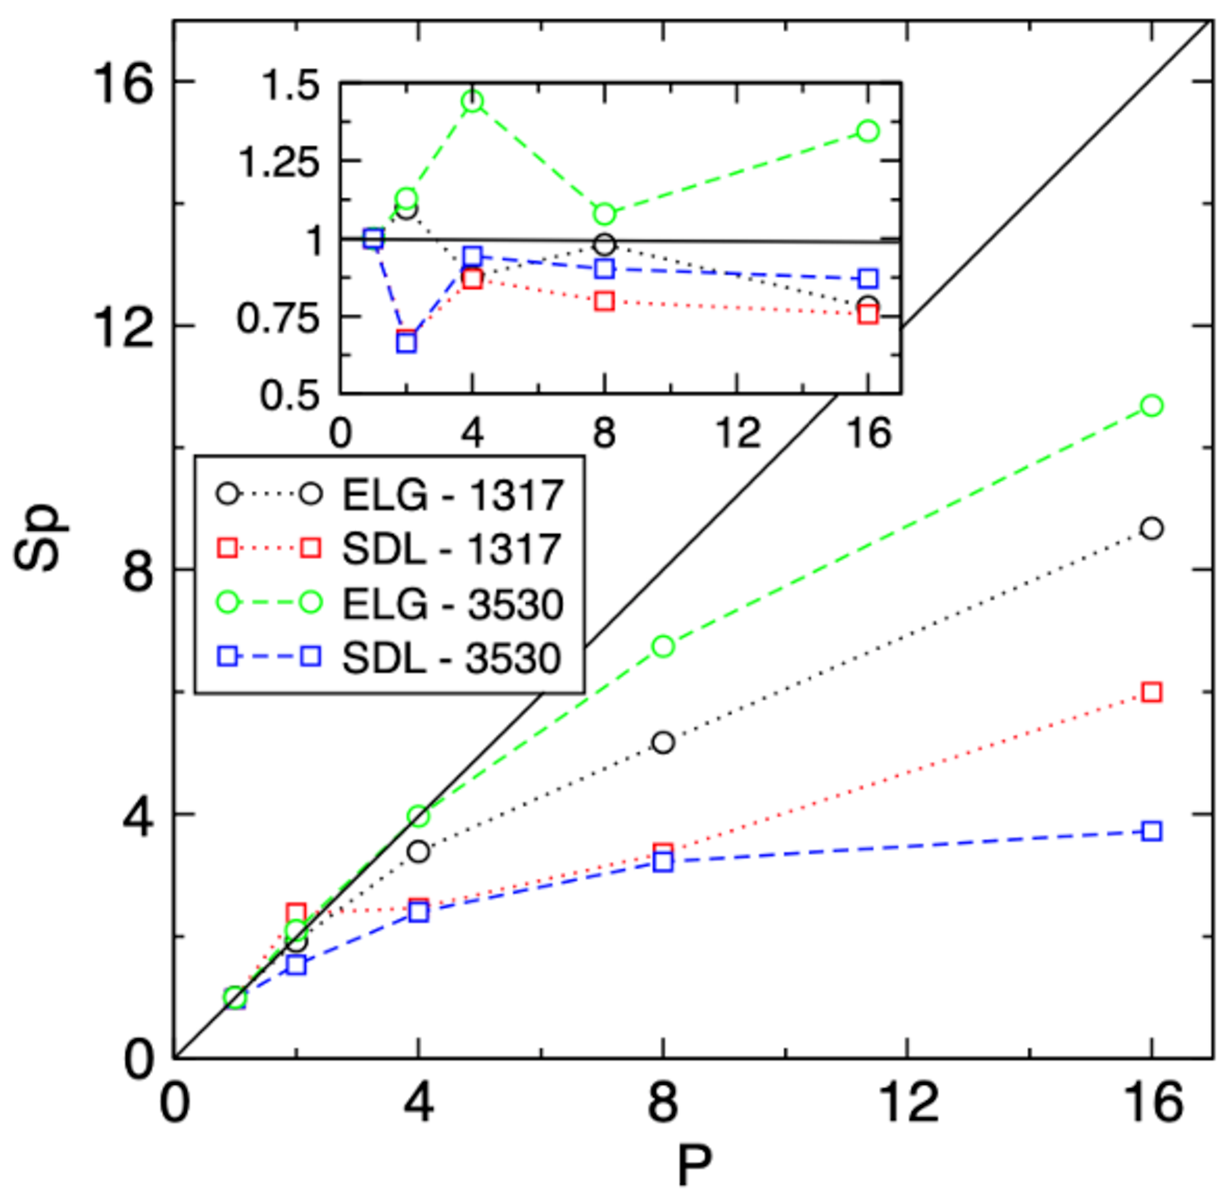
\includegraphics[width=0.5\linewidth]{figs/1_Scaling.pdf}
  \caption{Speed up scaling with number of cores}
\end{figure}

\section*{Compiling a parallel version of LMGC90}
To run simulations in parallel, you need to make a new compilation of LMGC90. Below, You will find a comparative step-by-step procedure on how to compile and run a single processor simulation and a multithreading simulation. 

Just for your information, there are several methods to run algorithms in parallel. LMGC90 uses an implementation called OpenMP.

\subsection*{Single processor}
\begin{enumerate}
  \item Open a terminal and go to your the directory containing the sources lmgc90\_user\_xxx.
  \item Type on your terminal:
  \begin{tcolorbox}
  \texttt{mkdir build} \\
  \texttt{cd build} \\
  \texttt{cmake ..} \\
  \texttt{make}
  \end{tcolorbox}
\end{enumerate}

\subsection*{Multi processor}
\begin{enumerate}
  \item Open a terminal and go to your the directory containing the sources lmgc90\_user\_xxx.
  \item Type on your terminal:
  \begin{tcolorbox}
  \texttt{mkdir build\_parallel} \\
  \texttt{cd build\_parallel} \\
  \texttt{cmake .. -DWITH\_OPENMP=True} \\
  \texttt{make}
  \end{tcolorbox}
\end{enumerate}

Now you have 2 installations of LMGC90 in your system. 
It is very important to differentiate each one when you want to run a simulation. 

Before, you have set your system to automatically recognize your installation with these lines (see compilation instructions in the lmgc90 wiki page): 

\begin{tcolorbox}[colback=blue!10]
\begin{verbatim}
  if [ -z ${PYTHONPATH} ]; then
    export PYTHONPATH=mysourcepath/build
  else
    export PYTHONPATH=${PYTHONPATH}:mysourcepath/build
  fi
  export PATH=${PATH}:mysourcepath/src/addons
\end{verbatim}
\end{tcolorbox}

\textbf{To run a single-processor simulation}, you have to write on the terminal (before running your scripts) the line corresponding to: 

\begin{tcolorbox}
\begin{verbatim}
  export PYTHONPATH=${PYTHONPATH}:yoursourcepath/build
\end{verbatim}
\end{tcolorbox}

\textbf{To run a multithreading simulation}, you first need to write on the terminal these two lines:

\begin{tcolorbox}
  \begin{verbatim}
    export OMP_SCHEDULE=STATIC
    export OMP_NUM_THREADS=4
\end{verbatim}
\end{tcolorbox}

The first line sets that you will be using a given number of processors, and you do not allow the algorithm to use more than that. 

asda sd s fsd gffsd fsdfds

The second line sets the number of processors that you want to use. 
In this example, we set the number of processors to 4. 

Then, you have you set your PYTHONPATH to the multithreading compilation. Something like: 

\small
\begin{tcolorbox}
\begin{verbatim}
export PYTHONPATH=${PYTHONPATH}:yoursourcepath/build_parallel
\end{verbatim}
\end{tcolorbox}
\normalsize

And then you can run your scripts normally. 
You can also check on your computer tasks manager the number of processors your script is using. 
It can vary between 1 and the number of processors max (OMP\_NUM\_THREADS) that you set, depending on the routines the code is running at that moment. 

\end{document}
